%%%%%%%%%%%%%%%%%%%%%%%%%% Proposal of the first year %%%%%%%%%%%%%
\documentclass[a4paper,11pt, english]{article}

%%%%%%%%%%%% Packages
\usepackage[table]{xcolor}         			% colored text
\usepackage{smartdiagram}
\usepackage{adjustbox}
\usepackage{changepage}
\usepackage{standalone}
\usepackage[utf8]{inputenc}
\usepackage{hyperref}
\usepackage{lipsum,calc}
\usepackage{array,longtable}
\usepackage{tabularx} 
\usepackage{collcell}
\usepackage{pgfplots}
\usepackage{graphicx}
\usepackage[all]{xy}         			% diagrams
\usepackage{amssymb}				% \mathbb and others
\usepackage{amsthm}				% theorem styles
\usepackage{amsmath}				% Declare math operator
\usepackage{enumerate}       			% many possible numerations
\usepackage{manfnt,xspace}			%% added package
\usepackage[a4paper,top=3cm, bottom=3cm, left=3cm, right=3cm]{geometry}
\usepackage{pifont}% http://ctan.org/pkg/pifont
%\usepackage{natbib}


%\usepackage[backend=bibtex,style=numeric,citestyle=numeric]{biblatex}
\usepackage[backend=bibtex,maxbibnames=99]{biblatex}

\addbibresource{proposal_correct}
                        

\newcommand{\cmark}{\ding{51}}                    
                        
\definecolor{lightgreen}{HTML}{CCFF66}
\definecolor{green}{HTML}{66FF66}
\definecolor{lightyellow}{HTML}{FFFF66}
\definecolor{orange}{HTML}{FF9900}
\definecolor{red}{HTML}{FF3333}
\definecolor{cyan}{HTML}{00CCFF}
\definecolor{blue}{HTML}{0000FF}
\definecolor{blue-violet}{rgb}{0.54, 0.17, 0.89}
                        

%%%%% Font Macros
\usepackage{dsfont}
\usepackage[T1]{fontenc}
\def\lqq{{\fontencoding{T1}\selectfont\guillemotleft}}
\def\rqq{{\fontencoding{T1}\selectfont\guillemotright}}
\DeclareFontFamily{OT1}{pzc}{}
\DeclareFontShape{OT1}{pzc}{m}{it}{<->s*[1.10]pzcmi7t}{}
\DeclareMathAlphabet{\mathpzc}{OT1}{pzc}{m}{it}


\pgfplotsset{compat=1.9}

%%%%%%%%%%%%%%%%%%%%%%% title

\title{\vspace{0cm}
\hrule
\vspace{1cm}
\centerline{\LARGE{Thesis Proposal:}}
\vspace{0.5cm}
\centerline{\LARGE {\bf The Role of Embeddings in Data-Driven Augmentation}}
%\centerline{\LARGE{\bf }}
}

%\title{\begin{Large}Research Proposal\end{Large}}
\author{Federico Dassereto}
\date{\today}

%%%%%%%%%%%%%%%%%%%%%%%%%%%%%%%%%%%%%%%%% DOCUMENT %%%%%%%%%%%%%%%%%%%%%%%%%%%%%%%%%%%%%%%%%%%

\begin{document}
\maketitle
\hrule 
\vspace{1cm}

\begin{abstract}
    %A-o meu neuo gh'é neue nae neue: a ciù neua de neue nae neue a n'eu anâ.    
    Querying data lakes containing a large amount of unstructured data is a difficult task, accentuated by the facility of producing data due to the rise of the World Wide Web. A traditional operation on data lakes is to search for joinable and unionable tables, in order to find tables related to specific user requests. Existing approaches search for columns with the best overlap possible, returning columns from tables in data lakes with high joining or unionability rating. These approaches fail to capture the situation in which a data scientist wants to find related tables related to a particular query table, when she is trying to build a machine learning model to predict a column of her query table. The reason for which existing approaches fail is that they do not consider the impact that a joining table has on the predicting tasks, due to the lack of semantic surrounding the data lake. 

    The goal of the thesis is to define an automatic table augmentation framework, to improve the performance of machine learning models in predicting target columns of a query table. The idea is to start by studying the augmentation problem as a problem on data lakes only, with measures and concepts derived from information theory and functional dependencies, and then integration embeddings in the process. Embeddings will be integrated by mapping tables to knowledge bases and exploiting their semantics to automatically produce the augmentation. More precisely, the thesis will first propose a framework for automatic horizontal table augmentation in data lakes, allowing a data scientist to add relevant features to her query table from a ranking of joining tables. Furthermore, an extension comprehending a mapping of tables to knowledge bases and exploiting knowledge bases embeddings will be developed, in order to study the role of embeddings in automatic tables augmentation. Finally, to sum up the previous results, an ad-hoc embedding algorithm for knowledge bases will be developed to to emphasize the relevant properties a knowledge base should have to produce a relevant augmentation.
\end{abstract}

\section{Motivation and Description}\label{motivations}

Since the rise of the World Wide Web, we have experienced an exponential growth in publicly available data. Data has become a crucial element in everyday life and many devices continuously produce and store them in a forest of different formats. This exponential growth has posed many challenges to scientists (even going so far as to create the figure of the \textit{data scientist}) in every step in which data are traditionally used: from data collection to integration, from processing to visualization. The impact of \textit{Big Data} has been summarized in \cite{mcafee2012big}, where the key properties are \textbf{V}olume, \textbf{V}elocity, \textbf{V}ariety, \textbf{V}eracity and \textbf{V}alue. 

In data science, it is increasingly the case that the main challenge is not in integrating known data, rather it is in finding the right data to solve a given data science problem. Today, data is a mass (uncountable) like dust, and data surrounds us like dust, even lovely structured data. Data is so cheap and easy to obtain that it is no longer important to always get the integration right and integrations are not static things (\textbf{V}elocity component). Data integration research has embraced and prospered by using approximation and machine learning. The uncontrolled nature of data manifests in large repositories of data (data lakes), in which both structured and unstructured data are stored. The peculiarity of data lakes lies in the fact that there is uncertainty about the presence of metadata describing the data themself. Furthermore, it is common the situation in which there is a lack of schemas, making traditional database approaches to integrating or querying data difficult to pursuit or even infeasible. Along with the uncertainty regarding the quality of the data, the amount of such data makes it infeasible also the traditional human-in-the-loop framework, since hand-labeling or manual rating of very large amounts of data is extremely expensive. It is easy to see that searching in data lakes is a complicated task, both in terms of time and methodology. 

Following the path traced by Tim Berners-Lee et al. in \cite{bizer2011linked} about Open Data publication and maintenance, many organizations are publishing data, augmentating tremendously the \textbf{V}olume and the \textbf{V}alue of such data. On the other hand, the explosion of sources providing data increases their \textbf{V}ariety, requiring new techniques to integrate data.
At a processing level, the main difficult arisen by the multiple sources and possibly unstructured data is given by the interpretation, i.e., the semantic layer. To extract semantics from unstructured data, in the last years the concept of embedding has been proposed. Embeddings are predominantly used in learning representations of texts \cite{mikolov2013efficient} and graphs \cite{nickel2017poincare}. In the last year, an approach exploting embedding to solve data integration task \cite{cappuzzo2020creating} has been published. This work can be seen as forerunner for the integration of embeddings in data management tasks, even if it works on tables from the same context.

A data scientist who is trying to solve machine learning tasks, frequently found herself in the situation in which there are not enough data to build a good model. Given the amount of data previously discussed, it would be very useful a framework which enables her to find automatically new features or samples to improve the model. Broadly, two main classes of augmentation can be distinguished: \textit{Horizontal Augmentation}, in which new significant features are added to the dataset and \textit{Vertical Augmentation}, in which new samples (tuples) are added to the dataset. Ideally, the two classes can be seen as the search for joinable (Horizontal) or unionable (Vertical) tables in the data lakes situation, and Knowledge Bases (KB) completion or extensions (vertical).

In this thesis, we focus on the problem of \textit{using embeddings for automatic augmentation of data to improve machine learning tasks}. We believe that it is a crucial integration task that has not yet been explored, either as augmentation problem itself nor with the usage of embeddings. Few approaches that try to augment tables with respect to a repository have been proposed; the two closest approaches proposed until now show different problems: (i) a set of rules to decide if it is safe to avoid a join or not \cite{kumar2016join}, restricted to a \textit{pure relational} settings, i.e., the schemas of each table is known; and (ii) a feature selection algorithm working on a matrix in which the number of attributes is much larger than the number of tuples \cite{chepurko2020arda}. 

The goal of this thesis is to study how to stabilize the automatic increase and make it scalable to possibly huge tables or data lakes. The idea is to define indexing structures, based on information theoretic measures, to make the search for joining tables fast and adapt to the variety of existing joining possibilities (one-to-one, one-to-many, many-to-one, many-to-many). More precisely, the thesis will proposed and index for horizontal augmentation on the data lakes scenario, as well as the integration of embeddings in the augmentation of KBs. Eventually, an embedding algorithm for KBs will summarize unified framework the two previous results.






\section{Reference Area and Relevance of Goals}\label{reference}
To the best of our knowledge, no automatic table augmentation framework adapt to work at Internet Scale exists. We believe that such a framework would be very relevant to exploit that large amount of unstructured data available on the web and on data lakes, allowing not only to improve machine learning models but also to retrieve semantic information from a variety of schemaless tables.
The proposal lies in the reference area "Data Augmentation to improve Machine Learning Tasks", intending to provide to a data scientist an augmented set of data that enables her to improve model performances. The approach we propose differ from other existing solutions in the following aspects:
\begin{itemize}
    \item Existing approaches mainly focus on predicting the usefulness of a join under the relational hypothesis, i.e., the schema information is known. To this end, we plan to develop an approach that is agnostic to the knowledge of the schemas.
    \item Existing approaches that try to augment data against a repository perform very expensive joins, and are evaluated concerning repositories of limited size; other existing approaches on repositories run features selection algorithms on a very large matrix derived by the join of all the joinable tables. To this end, we plan to develop an approach that does not materialize any kind of join and is scalable to hundreds of thousands of tables in a repository.
    \item Existing approaches on single tables identify the most relevant features in the table, according to a specific target. We plan to overcome the single table assumption by indexing all the tables in a repository and identifying the most relevant features, and the relative tables, that improve the machine learning model performances.
    \item Other approaches simply return the set of joinable tables, usually with a threshold to allow for relaxed  (imperfect) join, without any ranking. We plan to rank the returned tables according to the improvement that each of them will guarantee to the model.
\end{itemize}    

\section{State of the Art}\label{related}
In this section, we present related work that we consider relevant for the proposed research project. In order to facilitate reading, the discussion has been organized into fuor main sections, corresponding to the main concepts introduced in Section \ref{motivations} and \ref{reference}. Each of the four sections is in turn divided into sub-parts to further facilitate reading. The first one discusses embeddings approaches and their relevance to the proposal, the second introduces Open Data and their common operations, the third provides an overview of existing augmentation approaches and finally the fourth reviews functional dependencies discovery approaches.

\subsection{Embeddings}

\subsection{Open Data}

\subsection{Augmentation Approaches}

\subsection{Functional Dependencies}

\section{Goals, Methodology and Preliminaries}\label{goals}
% In this section, we start with an highlight of the macro goals of the thesis, then we expand the content of Section \ref{motivations} by detailing our specific goals and the feasibility of each of them. Finally, we summarize the work done in the first year concerning the proposed goals.

In this section, we expand the content of Section \ref{motivations} by detailing our specific goals and the feasibility of each of them, by detailing the methodologies we plan to follow. Finally, we summarize the work done in the first year concerning the proposed goals.


\subsection{Goals}\label{sub_goals}
% The high-level goals of this thesis are:
% \begin{itemize}
%     \item To show the relevant role that embeddings can play in augmentation tasks;
%     \item To show that embeddings can be directly used to answer queries instead of being an orthogonal part of the answering process.
% \end{itemize}

The overall goal of this research proposal is the study of the role of embeddings in data augmentation, from tables augmentation on data lakes to an embedding algorithm for knowledge bases, passing through the integration of embeddings in existing tables augmentation framework exploiting knowledge bases. We organize the work into three main objectives, each leading to specific results. 
The aim of Objective 1 (\textit{indexing data lakes to augment}) is to analyze the state of the art on (i) open data search, and (ii) sketching and approximation of information-theoretic measures, and to define, implement and evaluate an index for tables augmentation in data lakes based on information-theoretic measures. 
The aim of Objective 2 (\textit{augmenting via embedded knowledge bases}) is to analyze the state of the art approaches in knowledge bases representation and augmentation, along with their role in augmenting tables and integrating of embeddings in such approaches, and to define, implement and evaluate a framework that exploits embeddings of KBs for augmenting. 
Objective 3 (\textit{embedding knowledge bases}) aims at proposing an embedding algorithm for knowledge bases, by creating a mathematical structure that encapsulates relevant features for catching the bast augmentation possible, and implementing and evaluating the proposed algorithm. Along with the mentioned tasks, Objective 3 aims at (\textit{staying up-to-date on embeddings}), in order to stay up-to-date with the newest embedding technologies and algorithms. It is transversal and equally distributed over the three years since it is a very dynamic topic, and the knowledge gained in recent years on the subject would not be lost.  

\bigbreak

\noindent\textbf{Objective 1: Indexing data lakes to augment.}
\begin{enumerate}
    \item \textit{Analysis of the state of the art approaches} related to (i) open data searching and indexing, and (ii) information-theoretic measures approximation and sketching. There exist many frameworks aiming at searching on open data, for tasks such as joinability and unionability, implementing different techniques. Information-theoretic measures are very useful and, for large datasets, can require a lot of time to be computed. We plan to study how to approximate such measures as well as sketching them on a subset of the available data.
    \item \textit{Definition of an index for tables augmentation in data lakes} based on information-theoretic measures, taking advantage of existing indexing structures (e.g., inverted index) by storing the information about a table and its columns, along with information theory measures regarding columns. In such a way, exploiting the fast search offered by the index structures, it would be possible to retrieve joining columns. The key idea is that we will exploit information-theoretic measures to simulate the behavior of functional dependencies. 
    \item \textit{Implementation and Evaluation of the index for tables augmentation in data lakes} on different data lakes scenarios and workloads, aiming at clarifying the usefulness of such an index.
\end{enumerate}


\noindent\textbf{Objective 2: Augmenting via embedded knowledge bases.}
\begin{enumerate}
    \item \textit{Analysis of the state of the art approaches} for knowledge bases construction, representation, and augmentation, along with their embedding algorithms. Since the variety of knowledge bases available, often built available as knowledge graphs, this analysis will be deeply and sharply isolate the fundamental features that a KB is required to have.
    \item \textit{Definition of a framework that exploits knowledge bases embedding to augment}, by understanding how embeddings algorithms works on knowledge bases and find the best possible representation to maximize the augmentation. Knowledge bases semantics can be very useful in extending tables, by adding not only features to maximize the augmentation but also to add new relevant tuples. Once the augmentation through embeddings will be completed, a comparison between with and without embedding approaches will be conducted, in order to highlight the key role of embeddings.
    \item \textit{Implementation and Evaluation of the framework for tables augmentation in data lakes with embeddings of knowledge bases}, by comparing the performances of this approach with respect to knowledge bases only and the index developed in objective 1.
\end{enumerate}

\noindent\textbf{Objective 3: Embedding knowledge bases.}
\begin{enumerate}
    \item \textit{Definition of an embedding algorithm for knowledge bases}, by representing in the best way the isolated relevant and general properties that KBs should have for being suitably embedded, along with an extensive evaluation on its efficiency compared to existing embedding techniques. To the best of our knowledge, in the state of the art of embedding algorithms, no algorithm exists that exploits the semantics of its entities, rather they exploit the structural properties of the knowledge base to project it onto a new semantic space. This objective will be founded on the results obtained in Objectives 1 and 2, in order to understand if embeddings effectively play a role. Since this objective is the farthest from the time of writing, not many details are reported.
    \item \textit{Implementation and Evaluation of the effectiveness of embedding algorithm} for knowledge bases, to show the relevance of this algorithm in knowledge bases representations and its impact on the quality of the augmentation.
    \item  \textit{Analysis of the state of the art approaches}, of continuously published embeddings works. Many embeddings approaches are yearly proposed, in a variety of formats: from completely new approaches to slightly changes on existing ones, from pre-trained embedding on large structures to new benchmarks. This objective includes the tracking of theoretical new ideas and implementations, in order to able to integrate new embeddings ideas in this work.
\end{enumerate}

% \noindent\textbf{Objective 4: Stay up-to-date on embedding techniques.}
% \begin{enumerate}
%     \item \textit{Analysis of the state of the art approaches}, of continuously published embeddings works. Many embeddings approaches are yearly proposed, in a variety of formats: from completely new approaches to slightly changes on existing ones, from pre-trained embedding on large structures to new benchmarks. This objective includes the tracking of theoretical new ideas and implementations, in order to able to integrate new embeddings ideas in this work.
% \end{enumerate}


\subsection{Methodology}\label{sub_methodology}
In the following, we describe the methodology we envision for achieving each objective described in Section \ref{sub_goals}.
\bigbreak

\noindent\textbf{Objective 1: Indexing data lakes to augment.}
\begin{enumerate}
    \item \textit{Analysis of the state of the art approaches} related to (i) open data searching and indexing, and (ii) information-theoretic measures approximation and sketching. We will review the most relevant solutions to open data problems, like table joinability and unionability, as well as the relevant results obtained in approximating and sketching information-theoretic measures. To this aim, we will take into account both the scientific literature related to data management and to data analysis and learning.
    \item \textit{Definition of an index for tables augmentation in data lakes} based on information-theoretic measures. We plan to propose an index for automatic table augmentation in data lakes. In particular, given a table $T$, a join column $t_j$ of $T$, a target column $t_y$ of $T$ and a data lake $D$ composed of $n$ tables ($D_1,...,D_n$), the index will return a ranking of tables in $D$, joining on $t_j$ that provides the best augmentation for $T$, i.e., mostly improves the performances of a machine learning model that has $t_y$ as target.
    \item \textit{Implementation and Evaluation of the index for tables augmentation in data lakes}. In order to show the relevance of our index, we plan to implement and evaluate it against different data lakes, taking into account the capability of producing accurate augmentations at reasonable times.
\end{enumerate}

\noindent\textbf{Objective 2: Augmenting via embedded knowledge bases.}
\begin{enumerate}
    \item \textit{Analysis of the state of the art approaches} for knowledge bases construction, representations, and augmentations. We will conduct a deep and complete analysis of the state of the art approaches and algorithms to manipulate and represent KBs, as well as embedding algorithms for KBs. The main distinction in the embedding approaches will be among the ones with a geometric interpretation, i.e., transitional operations between vectors and the ones based on matrix factorization and co-occurrences, i.e., the family of embedding closer to word embeddings.
    \item \textit{Definition of a framework that exploits knowledge bases embedding to augment}. In the case of semantic data lakes, i.e., data lakes with known (or derivable) mappings on KGs, embeddings can be exploited to retrieve relations between entities in the KG semantic space (for example through a nearest neighbors search or even more complex ways) and produce the augmentation. 
    \item \textit{Implementation and Evaluation of the framework for tables augmentation in data lakes with embeddings of knowledge bases}. Once the framework is designed and implemented, an evaluation of the two scenarios (augmenting via KGs only and KGs embedding) will be conducted to show the advantages of using embeddings. In such a situation, an augmentation using only KGs will be taken as baseline; it could work, in its simpler version, with a mapping from tables values to entities in the KG on which a basic join operation can be performed.
\end{enumerate}


\noindent\textbf{Objective 3: Embedding knowledge bases.}
\begin{enumerate}
    \item \textit{Definition of an embedding algorithm for knowledge bases}. Once Objective 2 is completed, we will have a picture of what features of existing KGs embedding have a positive impact on the augmentation and which one could be discarded on modified. To this aim, extensive knowledge of embedding algorithms will result in the definition of ad-hoc algorithms to embed KGs to provide table augmentation. The key concept for such an objective is that we do not want to propose a complete novel algorithm for embedding KBs, rather we plan to isolate and represent, in an appropriate way, the most important features of the KB to improve existing algorithms for KBs embeddings. In a sense, we want to integrate the semantic lying in the KB in the embedding process of existing algorithms, that up to now only consider structural properties.
    \item \textit{Implementation and Evaluation of the effectiveness of embedding algorithm} for knowledge bases. At such a point, a comparison between all of the approaches will be done: tables augmentation in data lakes only, table augmentation via KGs, table augmentation via KGs embeddings, and table augmentation via our KGs embedding algorithm.
    \item  \textit{Analysis of the state of the art approaches} of continuously published embeddings works. In order to review and keep track of the most relevant embedding approaches, the surveyed techniques we will then be organized into a taxonomy, according to their hypothesis, usage and domain of application.
\end{enumerate}



\subsection{Preliminaries}\label{sub_preliminaries}
In this section we will present the activities done and the results achieved in the first year.

\begin{figure}[t]\label{index_sketch}
    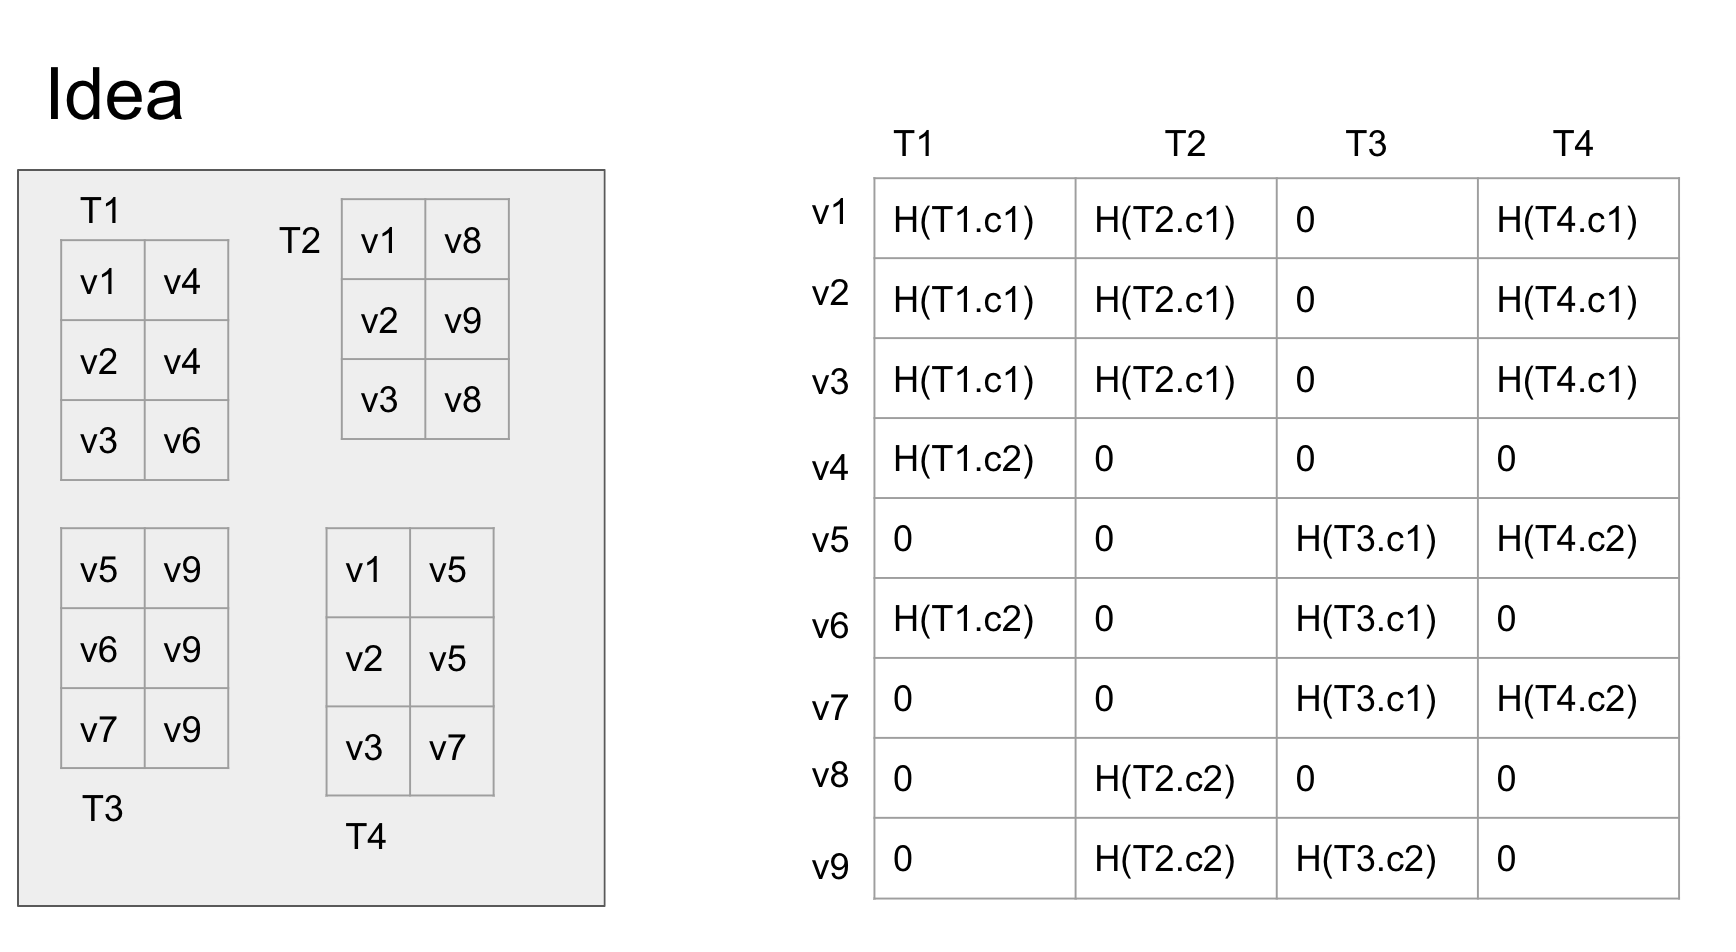
\includegraphics[scale=0.4]{figures/index_sketch.png}
    \caption{Sketch of entropy-based index for open data. When a value $v$ is present in column $j$ of table $i$, in position $(v,i)$ it is stored the entropy of the column of $j$ of table $i$.}
\end{figure}

\begin{enumerate}
    \item We have analyzed the state of the art approaches related to (i) open data searching and indexing, (ii) information-theoretic measures sketching and approximations, and (iii) functional dependencies discovery. We found out that existing searching frameworks on open data only cares about finding the best, or the best \textit{top-k} set, of \textit{joining} tables or columns. This has many drawbacks, first of which the fact that the best join does not say anything about the best augmentation. For example, the best join a table can have is with itself, which means a null increase.
    \item We also noticed that there are information-theoretic measures that are particularly suitable in representing, or at least approximating, the behavior of functional dependencies. In particular, the conditional entropy $H(Y|X) = H(X)-I(X,Y)$, where $H(X)$ in the Shannon entropy of variable $X$ and $I(X,Y)$ is the mutual information between variables $X$ and $Y$, has lower bound 0 and upper bound $H(X)$. These two cases coincides with full functional dependency\footnote{Note that, despite the differentiation that we made in Section \ref{related} about functional dependency, up to now the interpretation is the same on classical database FDs and descriptive FDs.} when $H(Y|X) = 0$ (meaning that the value of $Y$ is totally determined by $X$) and complete independence, when $H(Y|X) = H(Y)$ (meaning that the knowledge of variable $X$ has no impact on the knowledge of $Y$). This observation, mixed with the intuition that if a functional dependency (in its descriptive interpretation) between a set of attributes and a specific target holds these attributes are interesting for the augmentation, means that discovering FDs that minimize the conditional entropy\footnote{Actually, our intuition derived by the fraction of information, i.e., a normalized variant of the mutual information defined as $\frac{I(X;Y)}{H(X)}$. However, it is possible to show that minimizing the conditional entropy is equal to maximize the fraction of information.} produce the best augmentation. However, the approach of identifying a target attribute and discover FDs in such a way requires the materialization of the join, that, as discussed in Section \ref{related}, is unfeasible on data lakes.
    \item We also analyzed the role of Functional Dependencies (FDs). FDs express relationships between attributes of a database relation. An FD $X$ $\rightarrow$ $Y$ states that the values of attribute set X \textit{uniquely} determine the values of attribute $Y$. Despite their rich semantic information, functional dependencies are extremely hard to compute, as they belong to the W[2] complexity class \cite{blasius2017parameterized}. Particularly interesting are the non-trivial (FDs that cannot be derived from others) and minimal functional dependencies. Many works have been proposed to mine functional dependencies from tables: lattice-based approaches such as TANE \cite{huhtala1999tane} and DFD \cite{abedjan2014dfd} that performs search and pruning on the lattice structure; row-based methods derive candidate FDs from two attribute subsets, namely agree sets and difference-sets, which are built by comparing the values of attributes for all possible combinations of tuples pairs, such as DepMiner \cite{lopes2000efficient} and FastFD \cite{wyss2001fastfds}; incremental approaches exploiting the concepts of tuple partitions and monotonicity of FDs to avoid the re-scanning of the database \cite{wang2001incremental}. Of course, all of these approaches fail to scale to very large tables both in terms of time and memory usage. 

    We analyzed many of the above-mentioned FDs discovery algorithms, both exact and approximate, implemented in a popular framework named Metanome \cite{papenbrock2015data}. We found out, as expected, that no existing algorithm for FDs discovery is scalable to data lakes of thousands of tables and many Gigabytes of space. All of the experiments we run on single tables with thousands of rows and 30-40 attributes result in memory exceeding error or timeout. In sight of this, we chose to not follow the direction of pure FDs discovery, but to limit their usage to theoretical studies, such as upper and lower bounds studies and pruning techniques to improve our information-theoretic based index.
    
    The idea of inferring FDs from data has attracted a different view of such concept: the point of view change from \textit{uniquely implies} (roughly speaking, each left side of FDs is key with respect to the right side) to \textit{better identify} (each left side of FDs is a "substitute" of the right side). These kinds of FDs quantify how much the left side approximates the right side; it very useful in the situation in which correlations discovery and features elimination is needed. The mining of such an idea of FDs has been proposed by using information-theoretic measures like the reliable fraction of information \cite{mandros2017discovering} and the smoothed mutual information \cite{pennerath2020discovering}. The (partial) drawbacks of these last approaches are that (i) they require to know which variable the user wants to "describe", i.e., the right side of the functional dependency, and (ii) the right side must be composed of a single attribute, while the left side is generally made by several attributes. Furthermore, these approaches does not scale well with large tables with many attributes, while being able to manage table with many rows.
    
    \item To overcome the issue of the join materialization, we decided to exploit the idea of an inverted index, in which the information of each table is stored, along with each column entropy and the column-table association. The peculiarity of this index is that it looks like a sparse matrix, since all the unique values in all the tables are indexed, and the entropy information for each column is stored only when i-th values belong to j-th column. Figure \ref{index_sketch} shows a sketch of the designed index.
    \item We are currently working on the implementation of such an index, along with the research for understanding if mixing up the entropies is enough to simulate the conditional entropy behavior or a bit more elaborated metrics is required.
\end{enumerate}



\section{Research Plan}\label{researchplan}

We aim at organizing our research in the three years according to eight activities, listed in Table 1. Each activity corresponds to a thesis objective or to the thesis writing. In particular, Table \ref{table1}, for each activity, points out each sub-objective and the time units dedicated to it, while Table \ref{table2} presents their schedule in the three years.

% 1 Analysis of the state of the art on open data, sketching and approximation of information theory measures
% 2 Definition of an index for tables augmentation in data lakes based on information-theoretic measures
% 3 Analysis of the state of the art on functional dependency discovery algorithms

% 4 Analysis of knowledge bases representations and augmentations
% 5 Definition of a framework to include embeddings of knowledge bases in tables augmentation

% 6 Definition of an algorithm to embed knowledge bases
% 7 Evaluation of the performances of the knowledge bases embedding algorithm in answering queries

% 8 PhD thesis writing

\begin{table}[h!]\footnotesize
    \centering
    
    \caption{Workplan\label{table1}}
    \begin{tabular}{|c|p{9cm}|c|c|}
    \hline
    \textbf{Activity} & \textbf{Description} & \textbf{Months} & \textbf{Colour}\\ \hline
    1 & Analysis of the state of the art on open data, sketching and approximation of information theory measures & 1st Year & \cellcolor{lightgreen} \\\hline
    2 & Definition of an index for tables augmentation in data lakes based on information-theoretic measures& 1st Year & \cellcolor{green} \\\hline
    3 & Analysis of the state of the art on functional dependency discovery algorithms& 6 & \cellcolor{lightyellow} \\\hline
    4 & Analysis of knowledge bases representations and augmentations& 6 & \cellcolor{orange} \\\hline
    5 & Definition of a framework to include embeddings of knowledge bases in tables augmentation& 6 & \cellcolor{red} \\\hline
    6 & Definition of an algorithm to embed knowledge bases& 6 & \cellcolor{cyan} \\\hline
    7 & Evaluation of the performances of the knowledge bases embedding algorithm in answering queries& 6 & \cellcolor{blue} \\\hline
    8 & PhD thesis writing& 4 & \cellcolor{blue-violet} \\\hline
    \end{tabular}
    \end{table}
    
    \bigbreak
    \vspace{-2em}
    
    \newcolumntype{C}[1]{>{\centering\arraybackslash}m{#1}}
    %\begin{center}
    \begin{table}[h!]\footnotesize

    \caption{Workplan\label{table2}}
    \centering
    %\caption{{\bf A} = period abroad\label{table2}}
    
    \begin{adjustwidth}{-1.2cm}{}
    \begin{tabular}{|c|*{36}{C{.01cm}|}}%{|c|*{36}{p{.01cm}|}}
    \hline
    \textbf{Activity} & \multicolumn{12}{c|}{Year1} & \multicolumn{12}{c|}{Year2} & \multicolumn{12}{c|}{Year3} \\\hline
    %\cellcolor{orange}
                   1  &&&&&&&&&&&&&&&&&&&&&&&&&&&&&&&&&&&&\\\hline
                   2  &&&&&&&&&&&&&&&&&&&&&&&&&&&&&&&&&&&&\\\hline
                   3  &&&&&&&&&&&&&&&&&&&&&&&&&&&&&&&&&&&&\\\hline
                   4  &&&&&&&&&&&&&&&&&&&&&&&&&&&&&&&&&&&&\\\hline
                   5  &&&&&&&&&&&&&&&&&&&&&&&&&&&&&&&&&&&&\\\hline
                   6  &&&&&&&&&&&&&&&&&&&&&&&&&&&&&&&&&&&&\\\hline
                   7  &&&&&&&&&&&&&&&&&&&&&&&&&&&&&&&&&&&&\\\hline
                   8  &&&&&&&&&&&&&&&&&&&&&&&&&&&&&&&&&&&&\\\hline
    \end{tabular}
    \end{adjustwidth}
    \end{table}

\section*{Acknowledgements}{So long, and thanks for all the fish.}



%\nocite{*}
\printbibliography

\end{document}